%LyX 2.0.6 created this file.  For more info, see http://www.lyx.org/.
%Do not edit unless you really know what you are doing.
\documentclass[oneside,english]{amsart}
\usepackage[T1]{fontenc}
\usepackage[latin9]{inputenc}
\usepackage{amsthm}
\usepackage{fullpage}
\usepackage{graphicx}
%\usepackage{enumerate}
\usepackage{float}
\usepackage{amsmath}
\usepackage{url} % click on urls 

\usepackage[parfill]{parskip}
\usepackage{hyperref}
\usepackage{xcolor}

\usepackage{enumitem}

\makeatletter
%%%%%%%%%%%%%%%%%%%%%%%%%%%%%% Textclass specific LaTeX commands.
\numberwithin{equation}{section}
\numberwithin{figure}{section}

\makeatother

\usepackage{babel}
\begin{document}


\hspace{1cm} \\
\vspace{-3.5cm} 

\centerline{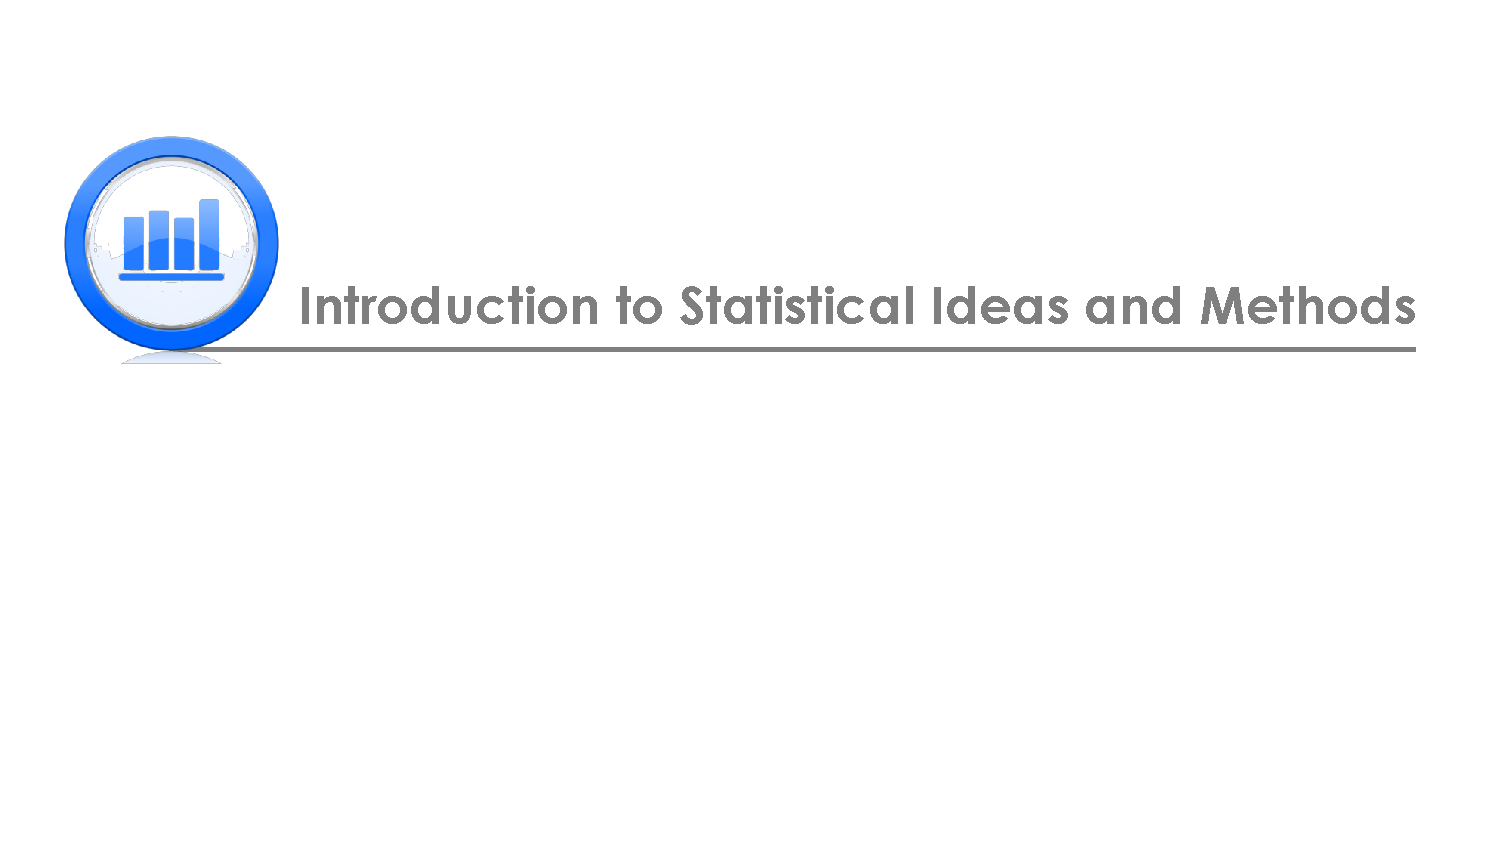
\includegraphics[width=1.1\textwidth]{../../figures/headerfinal.pdf}}

\vspace{.5cm}


%\centerline{{\large{Statistical Tests II: Power App}}} \normalsize  \vspace{.2cm} % Video title
\title{The Effective Use of Statistical Tests: Investigating Power Part 2}

\maketitle

The investigating power RShiny application illustrates basic power calculations for hypothesis testing in the proportions setting. 
The application has three main tabs corresponding to single sample testing (with user specified null hypothesis), two sample testing with equal sample sizes and 
two sample testing with unequal sample sizes. In this exercise we'll focus on the two sample case. Within each tab you may specify all of the values that affect the power of the corresponding test. These are:
\begin{itemize}
\item Sample size: the number of units in each group included in the study.
\item True probability for group A $p_A$: the actual probability of getting a ``yes'' response on a single trial in group A. For example, the true probability of seeing a heads on a single flip of a coin.
\item True probability for group B $p_B$: the actual probability of getting a ``yes'' response on a single trial in group A. For example, the true probability of seeing a heads on a single flip of a coin.
\item Alternative hypothesis: two-sided or directed one sided test.
\item Alpha: the significance level of the test.
\end{itemize}
The ``Power'' output gives the computed power for the specified sample size(s). The app also outputs a plot of power against sample size with the other user specified parameters held fixed.
Using the ``Comparison Plots'' subtab it is possible to plot additional power curves corresponding to different testing parameters. In this exercise we'll investigate power for only the single sample case.


In the previous exercise we studied a climate change scenario where we wanted to test if
the true proportion differs from some specific alternative. A more common
real world scenario is one where we'd like to compare proportions
in two different groups and we do not know the true value of the proportion
in either group. For example, in vaccine testing we might divide our
sample into a subset given the drug and a control group given a placebo;
then our task is to determine whether the proportion of people who
develop the associated disease differs between the two groups. Polio
is an infections disease that causes paralysis in a small proportion
of the people that it infects. Paralytic cases of this disease became
endemic in developed countries in the early to mid 20th century, particularly
in the United States in the 1950s. The development of the Polio vaccine
is widely considered one of the early triumphs of modern medicine
and the corresponding drug trial was one of the largest statistical
studies ever undertaken. With reference to the ``Equal Sample Size
Comparison'' tab of the RShiny application:
\begin{enumerate}
\item Suppose you have reason to believe that the true probability of contracting
Polio is $1\%$ without vaccination and $0.5\%$ with vaccination.
You want to run a drug trial to assess whether the vaccine is actually
effective. If your initial belief about the probability of contracting
Polio was correct, about how many people will you need to enroll in
the treatment group and the control group of your study to have at
least a $75\%$ chance of showing that the vaccine works? (Use $\alpha=0.05$)
\vspace{3cm}

\item Suppose instead of trying to show that the vaccinated group does better than the unvaccinated group you merely want to establish that the infection rate in the vaccination group is less than $1\%$.
This is a hypothesis test 
\begin{eqnarray*}
H_{0}:p & = & 0.01\\
H_{A}:p & < & 0.01
\end{eqnarray*}
in the single sample proportion setting. Using the same $n$ as in the previous
question and $\alpha=0.05$, what is the power of this test? Is it
the same as the power for the previous question? Explain why your
answer makes sense.
\vspace{3cm}
\end{enumerate}
Equal sample sizes are mathematically elegant but often difficult
to arrange in the real world. The unequal sample size comparison tab
treats the case where the two groups we are comparing have different
sample sizes.
\begin{enumerate}[resume]
\item It might be much easier to find people who haven't taken your Polio
vaccine than it is to convince people to take it. If this is true,
does it make sense to try to enroll the same number of people in the
group that takes the vaccine and the control group that doesn't? If
we enroll 5 times as many people in the control group as in the vaccine
group then how many people will we need to enroll in the vaccine group
to have a $75\%$ chance of rejecting the null hypothesis at the $\alpha=0.05$
confidence level?\end{enumerate}

\end{document}
